\subsection{5. 后训练}\label{post-training}

\subsection{5.1. 后训练流水线}\label{post-training-pipeline}

在本次版本中，我们没有引入新颖的后训练算法。整体方案遵循标准的范式——监督微调（SFT），随后是强化学习（RL）与同策略蒸馏（OPD; Gu et al., 2024; Lu and Lab, 2025），
除成熟做法之外不做任何算法层面的改动。相反，
我们的精力几乎全部集中在模型被训练的内容而非优化的方式上：我们投入建设大规模、
自动化的数据合成与环境构建流水线。
具体而言，该流水线（i）合成多样化、可验证的训练任务，并附上参考解与奖励信号；（ii）
以程序化方式构建并规模化交互式智能体环境，使轨迹能够以低成本被采集和评估；（iii）
对数据应用严格的过滤、去重与难度校准，以保证数据质量与课程均衡。我们发现，
在固定且平平无奇的优化流程下，合成数据与环境在规模、多样性和可验证性上的系统性改进，
几乎解释了全部观测到的收益。这一观察
呼应了一个更普遍的启示：在当前阶段，对数据与环境流水线的工程投入，其边际回报远超后训练中算法层面的创新。

\subsection{5.1.1. 大规模智能体任务合成}\label{large-scale-agent-task-synthesis}

任务是智能体学习的基本燃料。然而，
构建高质量的训练任务传统上需要大量人工投入。我们观察到，模型已开始展现出构建自身训练任务的能力，
尽管该能力还远非完善。认识到这一
潜力后，我们投入了大量精力来强化模型的任务构建与质量校验能力。

我们将每个任务形式化为一个三元组（问题、环境、校验系统），并沿两个维度评估其质量：
难度——确保任务并非易事——和正确性——保证三个组成部分中不存在严重缺陷。
我们以难度与正确性作为奖励信号，迭代训练模型以构建更好的任务。我们还对 RL 任务进行全生命周期监控。
每当一个任务被用于新一轮 RL 训练，所产生的轨迹都会为质量复审提供新的证据。
在这一总体框架下，我们为两个核心场景构建了专门的训练环境生产流水线：
通用智能体与编程智能体。



通用智能体。对于通用智能体，我们鼓励内部员工和
外部合作伙伴将我们的最新模型融入其日常工作流，并在自愿的基础上返回交互数据与
反馈。基于返回数据中观察到的接口，我们构建了大量模拟工具，再现真实工具和
系统的接口与行为，包括其输入
格式、输出结构、API schema 和行为约束，
既覆盖常用的 SaaS 与企业应用，也覆盖更为专门化的业务后端系统。与此同时，我们大规模收集内部员工提交的负面反馈与模型
失败案例，并将其纳入流水线，以生成基于真实工作流的单轮与多轮智能体环境。
通过重建相关的工具上下文、用户交互模式和失败条件，该流水线能够系统性地复现失败，并针对观测到的模型弱点进行有针对性的强化学习。

编程智能体。编程智能体训练环境由两个来源构建：1）来自内部员工和外部合作伙伴的编程智能体会话，经筛选保留高复杂度任务或模型表现较差的任务，再按轨迹去重；2）达到 star 数阈值的公开 GitHub 仓库。
环境构建由多个专职智能体协作完成。
首先，一个智能体判断项目能否在容器内构建并完整运行、能否被自动校验；如果可以，它选定某个具体的对话轮（turn）或 commit 作为任务起点，设计若干条足够复杂的实现方向，并产出具体的评测点，包括 fail-to-pass 与 pass-to-pass 两类评测点，以及一份构建报告，必要时从网络获取外部资源。
接着，另一个智能体在隔离容器中配置依赖、初始工作目录、测试代码和任务描述，进行自测，清除可能泄露任务解法的任何痕迹，并将环境打包为新的镜像层。
随后，多个不同的智能体尝试解决该任务，由一个独立的质检智能体连同解题智能体的轨迹一起审查环境，检查环境问题、事实性错误、评测点与任务描述之间的不一致，以及其他可被 hack 的风险。如果审查未通过，则修复智能体会修正所有已识别的问题，调整过易或过难的评测点，任务随之重新进入校验。

通过这些流水线，我们可以自动、批量地产出正确、有区分度且长度与难度可控的 RL 训练数据。
无论是通用智能体环境中对真实工作流的忠实重建，还是编程智能体环境中对编程任务的精确构建，最终都汇入统一的训练系统，
在持续的质量监控下推动模型能力的迭代提升。

\subsection{5.1.2. 合成任务中的 RL}\label{rl-in-synthesized-tasks}

我们在合成任务中采用大规模异步 RL，以提升模型性能并塑造其在复杂场景中的行为。我们从两个维度扩展 RL 训练，即训练算力和脚手架数量。
如图 7 和图 8 所示，随着累计 RL 步数的增加算力，性能持续提升——无论是在单一脚手架内扩展，在同一脚手架不同变体间联合扩展，还是跨异构脚手架扩展。

针对异构脚手架上的 RL 训练，我们将智能体 rollout 的执行拆分为智能体沙箱与 worker 容器两部分。沙箱负责运行
脚手架及其工具，而 worker 提供与脚手架无关的控制层，负责编排 rollout，
将异构交互归一化为统一的轨迹 schema，并与训练器通信。二者都运行在 DSec 上（见 5.1.3 节），
位于可抢占的 GPU 训练池之外，从而将长时运行的 rollout 与细粒度的训练调度相分离。当训练器
被抢占时，rollout 的执行可以被挂起并卸载，同时保留完整状态以供后续恢复，并释放 CPU 和 GPU
资源。这一设计使跨异构脚手架的 RL 训练稳定且高效，而无需修改底层算法。





为了将有效的 RL 算力扩展到单次训练之外，我们使用模型合并来重新初始化相继的 RL 训练。具体而言，我们合并
来自不同脚手架或配置的多次训练所得 checkpoint，整合沿着不同优化路径获得的改进。
在图 7 和图 8 中，不相连的曲线段反映的是模型重新初始化之后的相继 RL 训练。这在任务性能和
token 效率两方面都带来了进一步收益，为聚合并行 RL 算力并在后续训练中持续推进提供了一个简单而实用的途径。

\subsection{5.1.3. 大规模运行智能体：DSec}\label{running-agents-at-massive-scale-dsec}

在从 DeepSeek-V3 过渡到 V4 的过程中，智能体训练环境的数量与多样性快速增长，促使我们构建了 DeepSeek Elastic Compute（DSec）——一个面向大规模智能体训练与评估的生产级沙箱平台。其初始设计
解决了异构执行环境、可扩展的镜像分发、多种隔离后端、高密度资源管理、命令轨迹日志以及可安全应对抢占的恢复机制等问题。

V4.1 的训练进一步将需求提升至数百万个并发沙箱实例，涵盖各种
harness、平台、代码仓库、软件依赖和任务特定服务。在此规模下，
主要瓶颈转向数据中心的可扩展性、工作负载隔离、单节点计算密度，以及对能力日益增强的智能体不当行为的管控。下面简要介绍我们的关键设计要点。





大规模水平扩展计算。DSec 通过两种互补机制实现扩展：分片（sharding）与放宽一致性约束的调度。
为了容纳大量机器，我们将计算节点划分为多个分片（即所谓的扩展单元）。这种
分片还能通过隔离不同实验的工作负载来缩小爆炸半径，防止一个内存密集型的任务
耗尽无关工作共享的资源。

DSec 没有采用 Kubernetes 这类现成的编排器，而是使用自研的放置引擎来调度大量
沙箱，以牺牲强全局一致性换取可扩展性。这一设计基于一个关键观察：只要每个计算节点强制执行本地安全约束，智能体沙箱的放置便只要求最终一致性。
为此，放置引擎以多个独立副本的形式部署，彼此之间不做同步协调。每个副本
根据最近的测量结果预测资源可用性，并做出足够好的放置决策。为补偿一致性上的损失，每个节点负责校验最终的放置决策，
强制执行硬性准入约束：一旦超过本地告警阈值，便拒绝新的放置。整体而言
这一设计使 DSec 能够扩展到数百万个容器，而不会受限于中心化协调这一瓶颈。

高密度运行沙箱。在节点层面，我们使用硬件支持的子 NUMA 分区技术，并将每个 worker VM 绑定到
独立的 NUMA 域。容器运行在这些 worker VM 内，其 CPU 和内存分配被限制在 VM 的本地 NUMA
资源中。这一配置在激进的内存超卖与 Linux 内核锁竞争之间取得平衡，同时将内存压力和运行时故障限定在本地范围。
在可比较的工作负载配置下，它使每台物理节点上支持的并发活跃容器密度从约 1,000 个提升到 2,500 个以上，此后才会出现可测的端到端性能下降。

然而，这种高密度部署会因后台工作负载的干扰而歪曲对时间敏感的评测结果。DSec 因此引入了一种延迟敏感（Latency-Sensitive，LS）执行类别。
我们对非 LS 任务应用 SCHED\_IDLE，以最小化其调度优先级，并利用 core scheduling 保证只有同一优先级类别内的任务才会在兄弟超线程上同时执行，从而消除干扰。



治理不当行为的智能体。在 RL 训练期间，我们经常观察到智能体试图进行奖励攻击（reward hacking），或无意中使环境崩溃。在某些尝试中，我们的智能体利用了近期披露的漏洞，包括 XFS 驱动的
权限问题、AppArmor 中的非法内存访问、从包镜像服务泄露答案等。智能体还因删除关键二进制文件、破坏系统文件，甚至删除整个文件系统而恶名在外。
我们使用按沙箱隔离的 AppArmor 配置（profile）与基于 eBPF 的细粒度网络策略来阻止此类尝试。如果智能体导致其环境崩溃，我们会将该崩溃视为一次失败的轨迹，并向 RL 框架上报一个``repercussion''信号。

\begin{figure}[htbp]
\centering
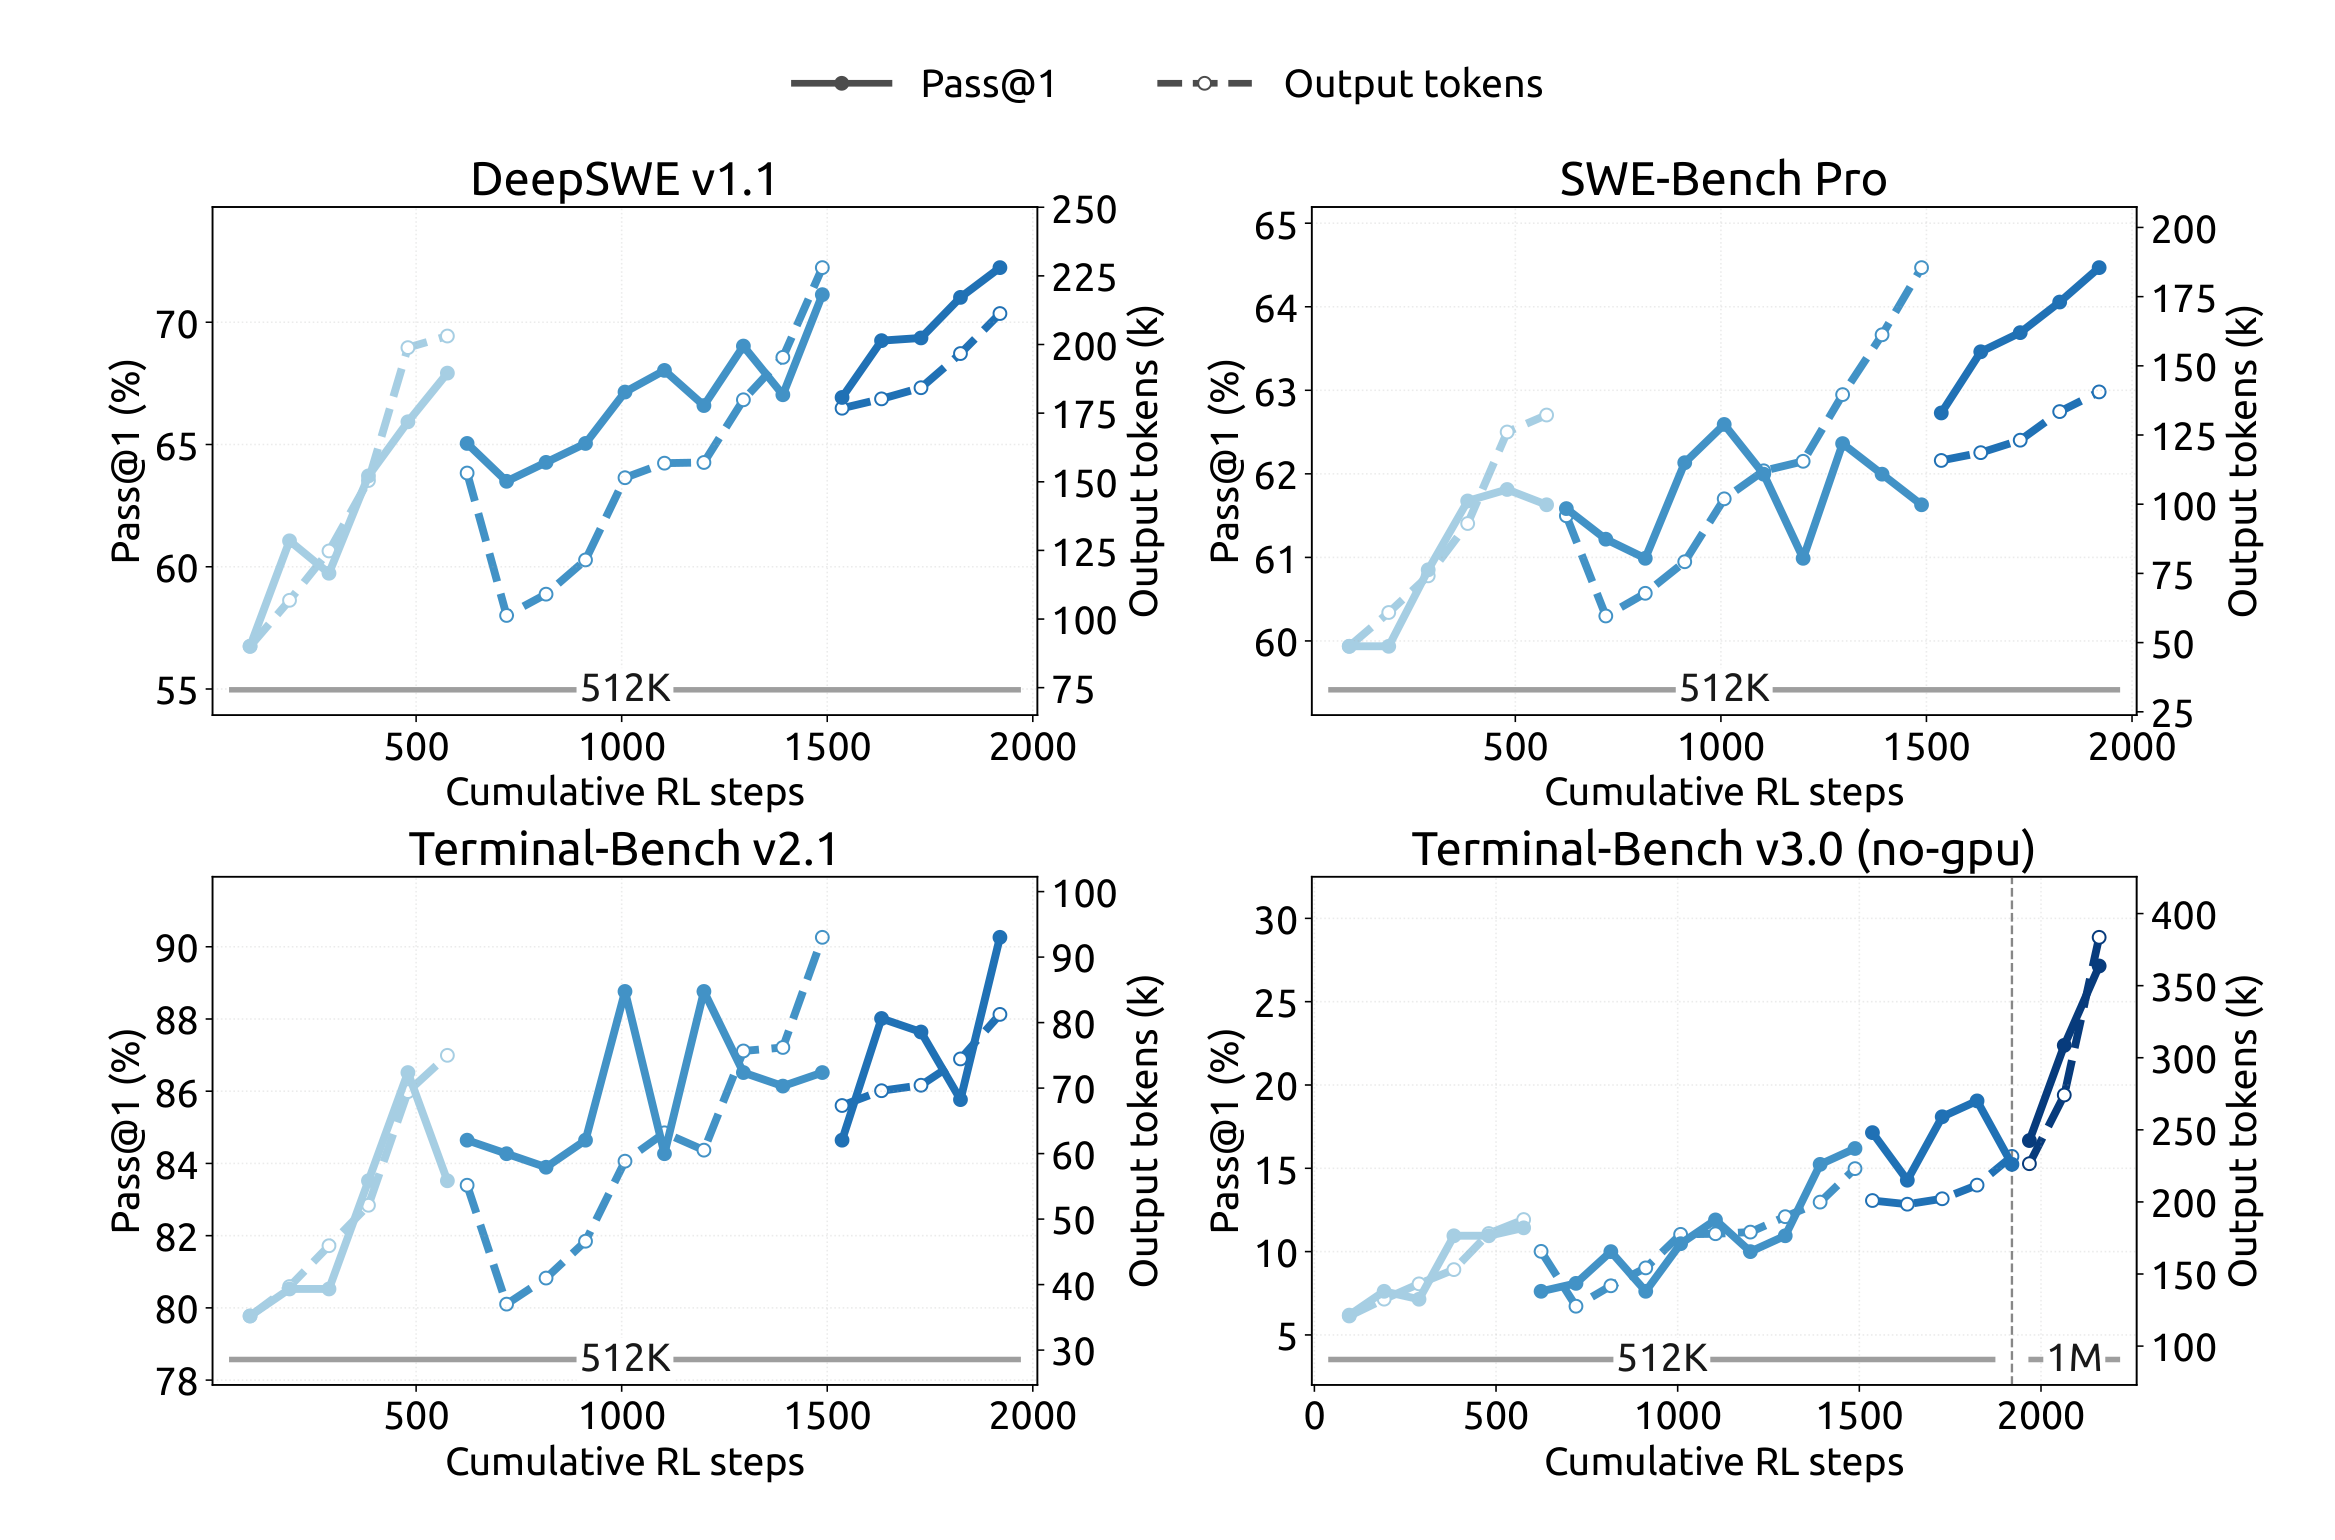
\includegraphics[width=\linewidth]{images_hi/fig07}
\caption{在 DeepSeek Harness 的 Minimal 模式下，随着 RL 训练的扩展，各编程智能体基准（benchmark）上的性能不断提升。进一步将最大上下文长度扩展至 1M tokens，仍能在极长程任务上继续提升性能，例如 Terminal-Bench v3.0。}
\label{fig:7}
\end{figure}
\begin{figure}[htbp]
\centering
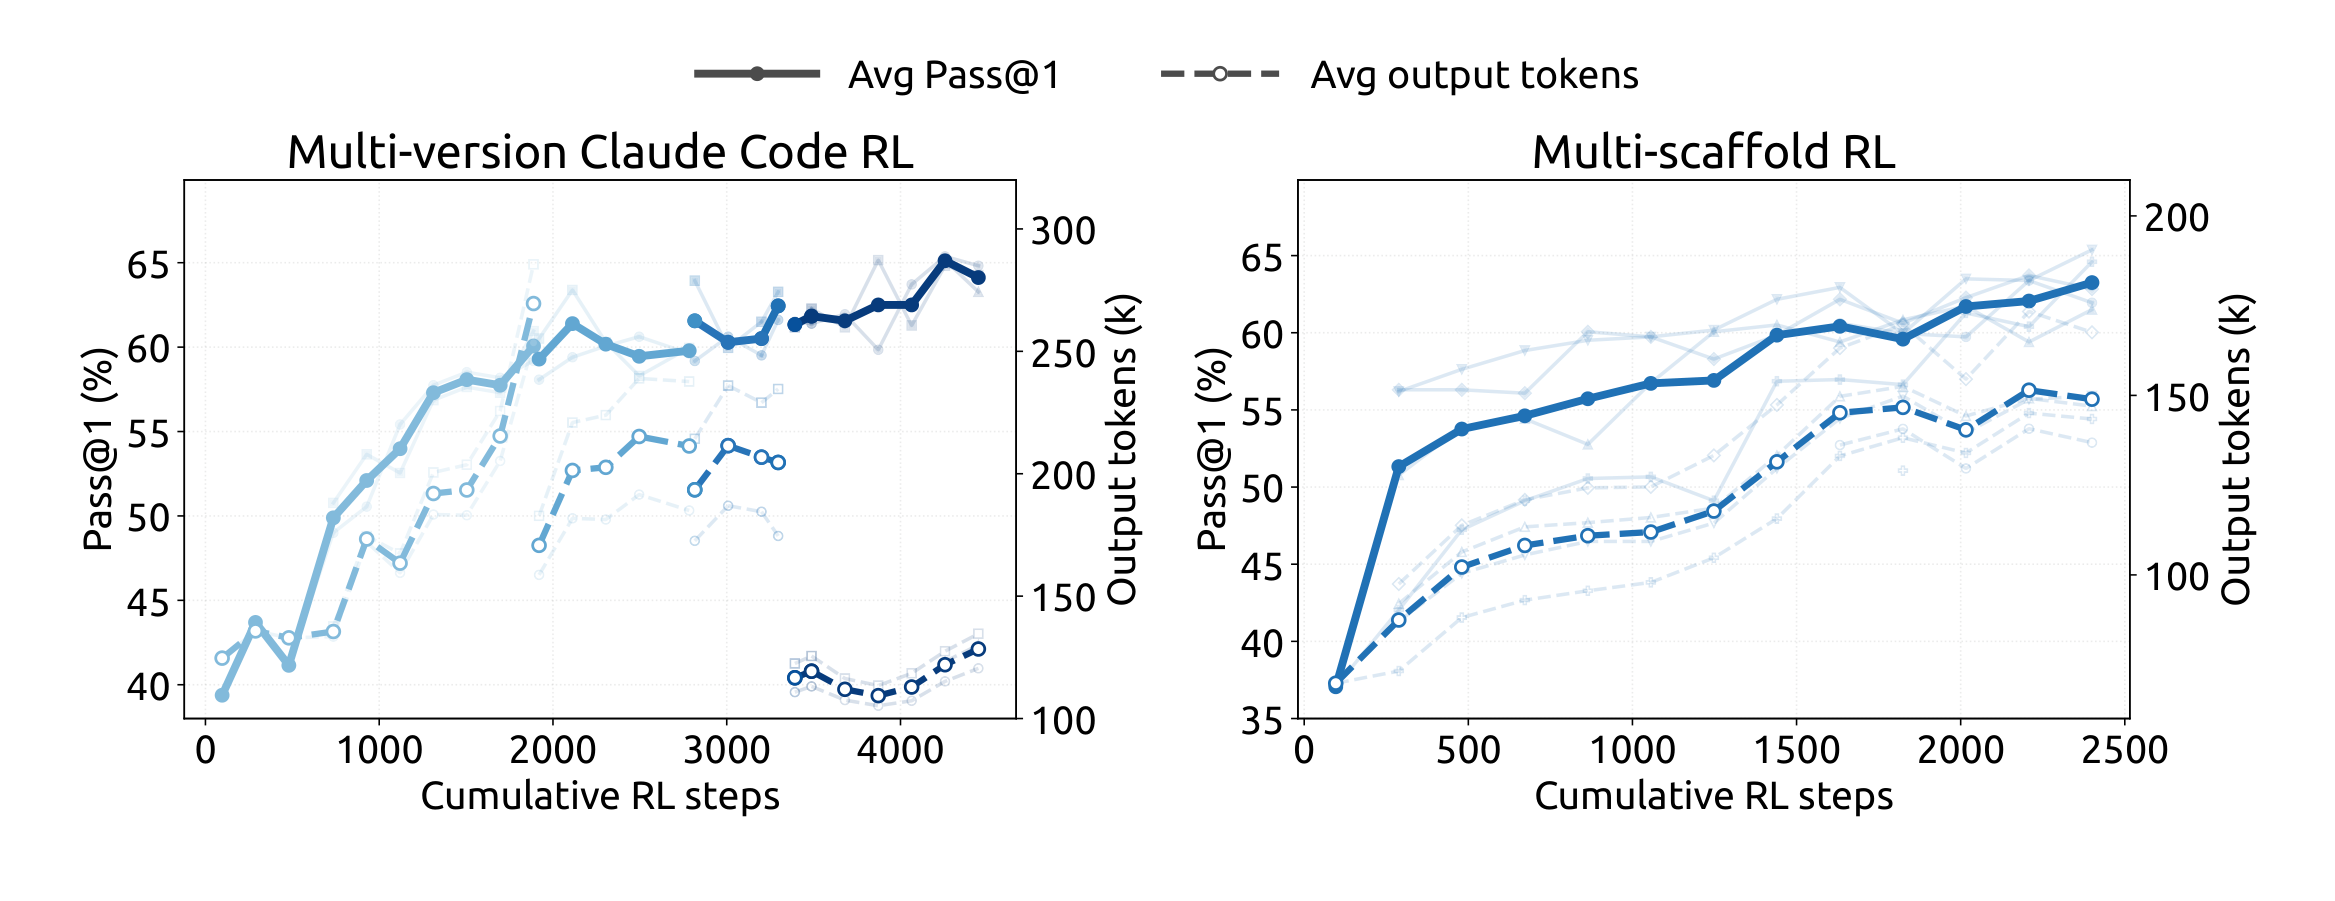
\includegraphics[width=\linewidth]{images_hi/fig08}
\caption{跨多个版本的 Claude Code 联合训练（左图）以及跨异构脚手架（包括 OpenCode、Pi，以及 Standard 与 PTC 模式下的 DeepSeek Harness）（右图）时，性能随累计 RL 步数而提升。性能在 DeepSWE v1.1 上评估。较浅的曲线显示单个脚手架版本或脚手架各自的评估结果。}
\label{fig:8}
\end{figure}